\documentclass[a4paper,12pt]{article} % добавить leqno в [] для нумерации слева
\usepackage[a4paper,top=1.3cm,bottom=2cm,left=1.5cm,right=1.5cm,marginparwidth=0.75cm]{geometry}
%%% Работа с русским языком
\usepackage{cmap}					% поиск в PDF
\usepackage{mathtext} 				% русские буквы в фомулах
\usepackage[T2A]{fontenc}			% кодировка
\usepackage[utf8]{inputenc}			% кодировка исходного текста
\usepackage[english,russian]{babel}	% локализация и переносы

\usepackage{graphicx}

\usepackage{wrapfig}
\usepackage{tabularx}

\usepackage{hyperref}
\usepackage[rgb]{xcolor}
\hypersetup{
colorlinks=true,urlcolor=blue
}
\usepackage{multirow}
\usepackage{hhline}


%%% Дополнительная работа с математикой
\usepackage{amsmath,amsfonts,amssymb,amsthm,mathtools} % AMS
\usepackage{icomma} % "Умная" запятая: $0,2$ --- число, $0, 2$ --- перечисление

%% Номера формул
\mathtoolsset{showonlyrefs=true} % Показывать номера только у тех формул, на которые есть \eqref{} в тексте.

%% Шрифты
\usepackage{euscript}	 % Шрифт Евклид
\usepackage{mathrsfs} % Красивый матшрифт

%% Свои команды
\DeclareMathOperator{\sgn}{\mathop{sgn}}

%% Перенос знаков в формулах (по Львовскому)
\newcommand*{\hm}[1]{#1\nobreak\discretionary{}
{\hbox{$\mathsurround=0pt #1$}}{}}

\begin{document}
	
	
	\vspace{4.5cm}
	{\huge
		\begin{center}
			{Лабораторная работа 18}\\
			Вибрационный магнитометр
		\end{center}
	}
	\begin{flushright}
		{\LARGE Салтыкова Дарья \\
			\vspace{0.5cm}
			Б04-104}
	\end{flushright}
	


\section*{{Введение}}
\subsection*{{Цель работы}}

Изучить основы конструирования и применения магнитометров с вибрирующим образцом для определения магнитных параметров как объемных образцов, так и тонких магнитных пленок.



\subsection*{Оборудование}

\begin{itemize}
    \item Вибропреобразователь(используется широкополосный динамик)
    \item Узкополосный фильтр
    \item Катушки малой индуктивности(используемые для приёма сигнала)
    \item Катушки большой индуктивности, используемые в качестве электромагнита
    \item Генератор сигналов 
    \item Синхронный детектор
\end{itemize}

\section*{{Методика}}

	Суть метода заключается в следующем: образец намагничивается постоянным магнитным полем зазоре электромагнита и одновременно приводится периодическое движение с низкой частотой. Поля рассеяния, обусловленные намагниченностью вибрирующего образца, создают осциллирующий магнитный поток в расположенной поблизости измерительной катушке. Согласно явлению электромагнитной индукции в катушке возникает переменное напряжение (ЭДС индукции). которое и является мерой намагниченности вещества (сравнивается с ЭДС от эталонного образца).
В нашей установке колебания происходят параллельно магнитному полю, а ось измерительных катушек (в количестве 2 штук) направлена перпендикулярно. \\ 


\noindent Важнейшим параметром магнитометров является чувствительность, т.е. минимальная величина магнитного момента, которую они могут устойчиво и воспроизводимо измерять. Установлено, что чувствительность зависит как от конструктивных особенностей, так и от экспериментальных условий. В связи с этим рассчитать оптимальную конструкцию с целью достижения заданной величины чувствительности весьма затруднительно.

\newpage

\section*{{Экспериментальная установка}}

\begin{figure}[htbp]
    \centering
    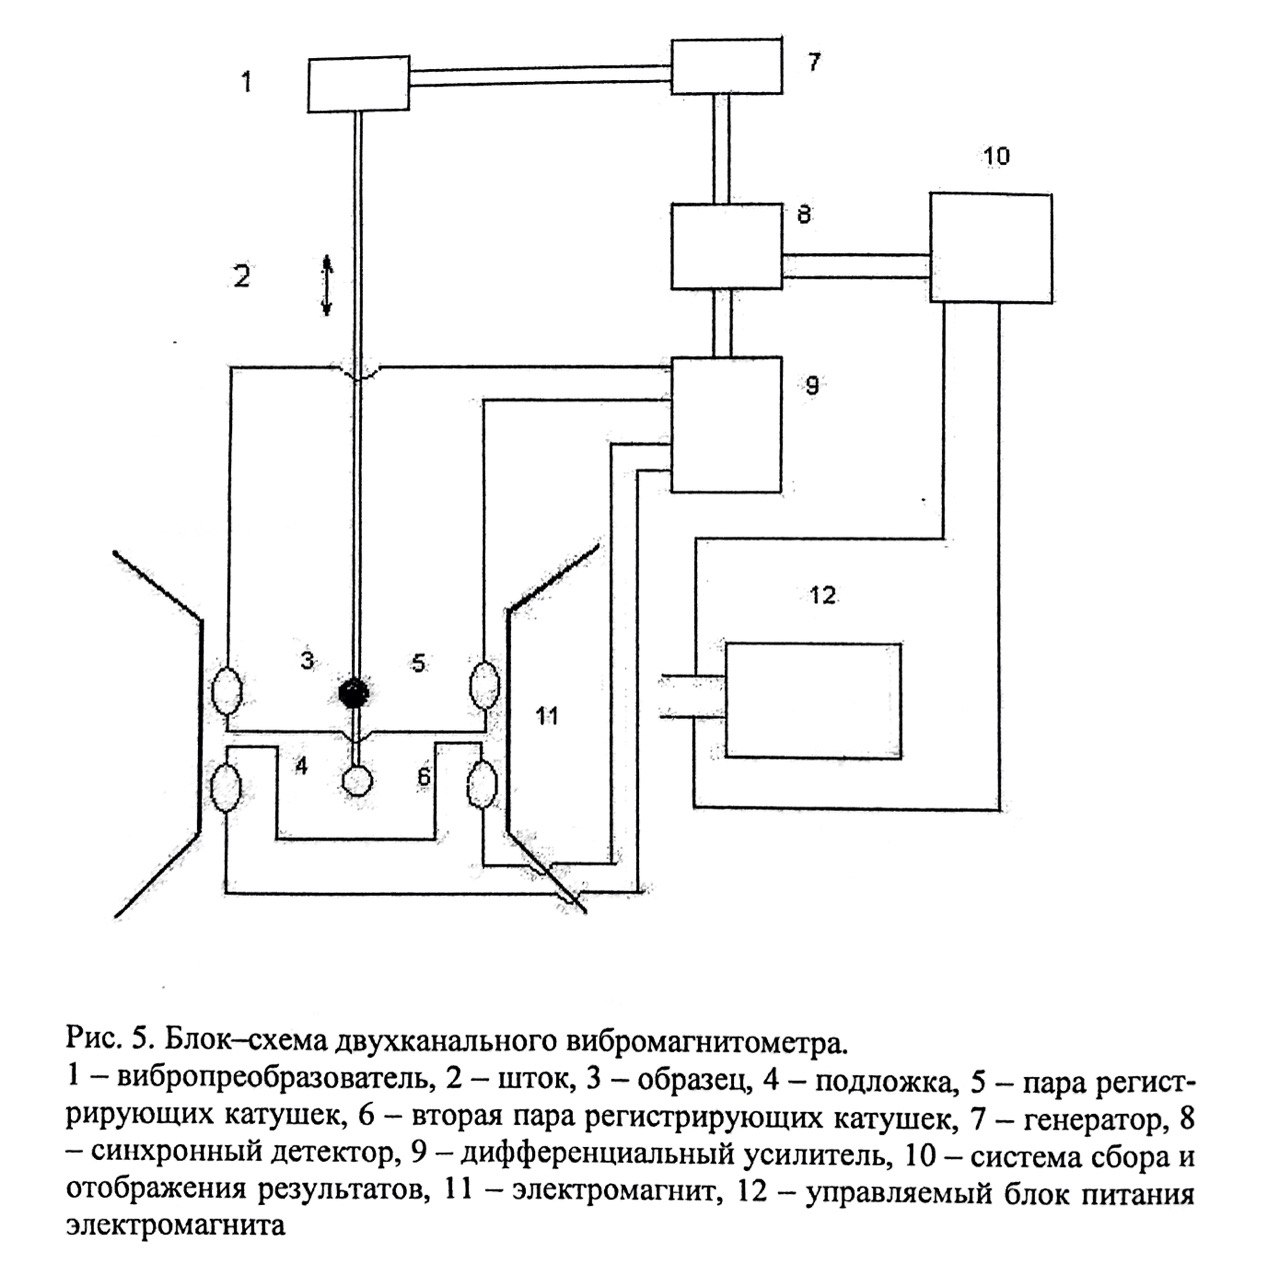
\includegraphics[width = 0.7\textwidth]{ustanovka.png}
    \caption{Схема экпериментальной устновки}
    \label{fig:setup}
\end{figure}



\section*{{Обработка экспериментальных данных}}

Измерим зависимость амплитуды выходного сигнала от частоты колебаний динамика. На рисунке видно \ref{fig:freq}, что наибольшая амплитуда достигается на частоте $\sim 36 \text{ Гц}$. Используем эту частоту для проведения дальнейших измерений. \\
\begin{figure}[htbp]
    \centering
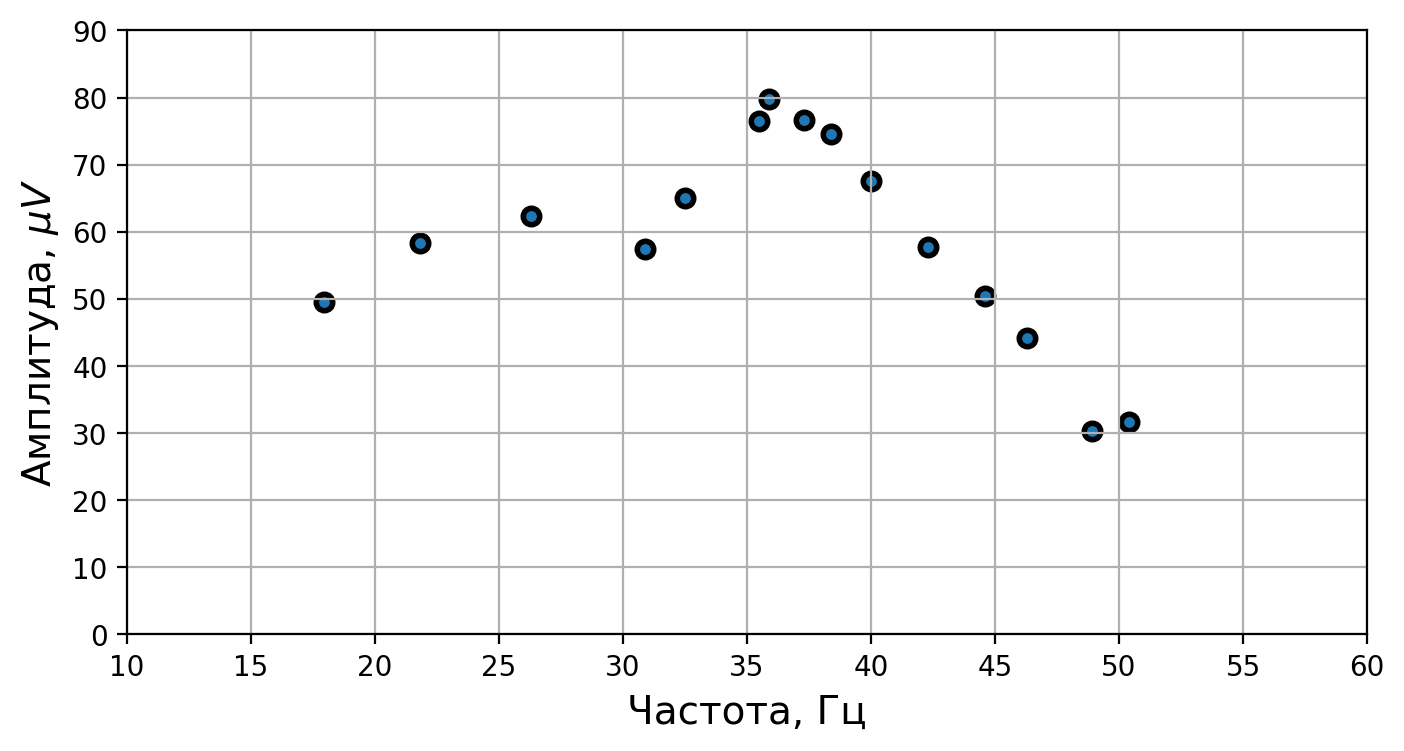
\includegraphics[width = 1.0 \textwidth]{freq.png}
    \caption{Подбор оптимальной частоты}
    \label{fig:freq}
\end{figure}


\noindent Снимем зависимость амплитуды выходного сигнала от силы тока, протекающего через катушки. \\
\begin{figure}[htbp]
    \centering
    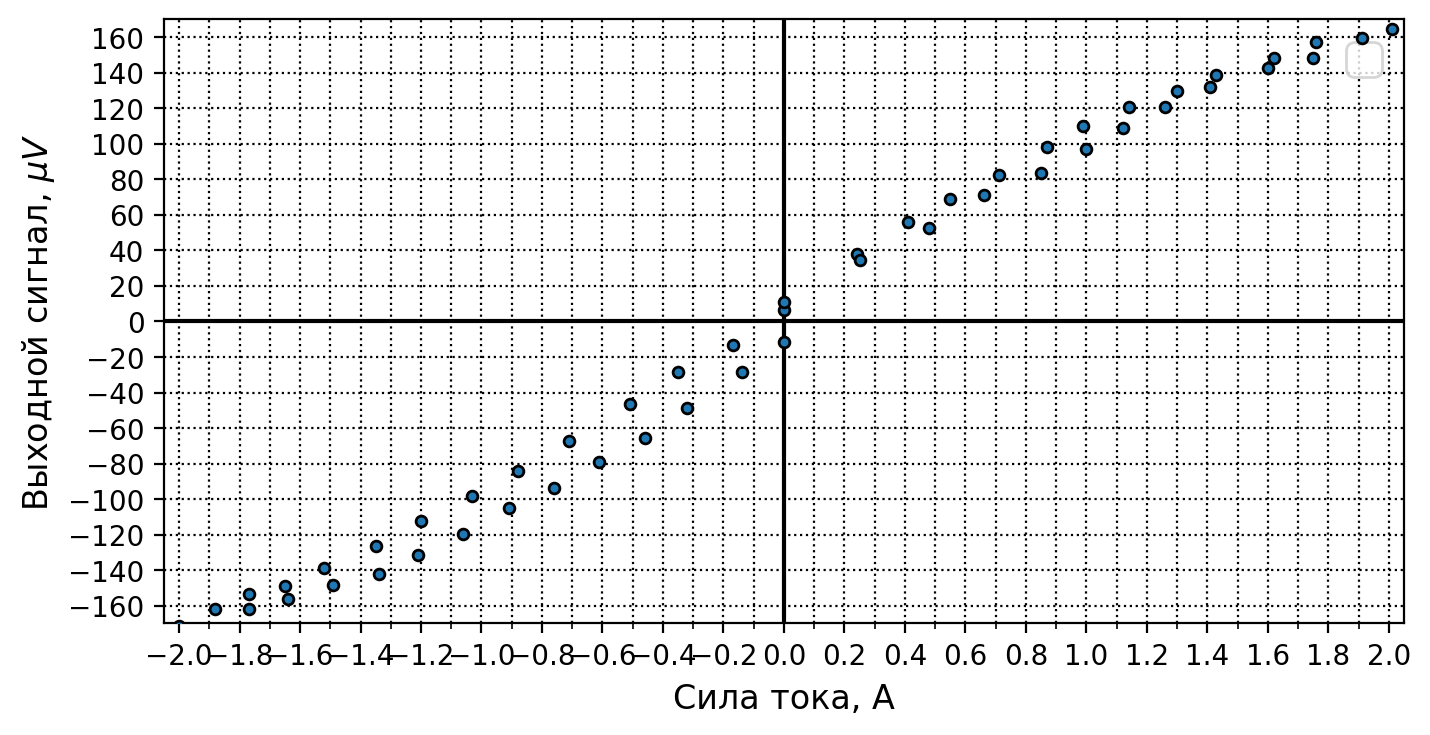
\includegraphics[width = 1.0 \textwidth]{magnetic_curve.png}
    \caption{Зависимость амплитуды выходного сигнала от силы тока, протекающего через катушки.}
    \label{fig:magnetic}
\end{figure}

\noindent Результаты измерений представлены на рис. \ref{fig:magnetic} - получен гистерезис. Поле, создаваемое катушками, пропорционально силе тока, который через них протекает. Магнитный момент образца пропорционален амплитуде выходного сигнала.

\section*{{Вывод}}

В ходе работы изучен принцип действия вибрационного магнитометра, а  также получено представление об использовании метода синхронного детектирования для обработкаи аналоговых сигналов. Сняты следующие зависимости: ЭДС индукции от частоты вибрации штока (рис. \ref{fig:freq}); ЭДС индукции от силы тока (рис \ref{fig:magnetic}).

\end{document}